\documentclass[tikz,border=3pt]{standalone}
\usetikzlibrary{arrows.meta}
\begin{document}
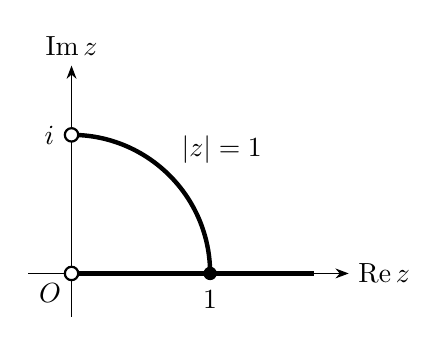
\begin{tikzpicture}[scale=1.1,>=Stealth,line width=0.9pt]
  % 座標軸
  \draw[line width=0.4pt,->] (-0.5,0) -- (3.2,0) node[right] {$\mathrm{Re}\,z$};
  \draw[line width=0.4pt,->] (0,-0.5) -- (0,2.4) node[above] {$\mathrm{Im}\,z$};

  % 対象領域のヒント：第1象限の単位円弧と正の実軸を太線で強調
  \draw[line width=1.6pt] (0,0) -- (2.8,0);
  \draw[line width=1.6pt] (1.6,0) arc[start angle=0,end angle=90,radius=1.6];

  % 含まれない端点（白丸）：z=0 と z=i
  \draw[fill=white,line width=0.8pt] (0,0) circle (2.2pt);
  \draw[fill=white,line width=0.8pt] (0,1.6) circle (2.2pt);
  % 含まれる交点（黒丸）：z=1
  \fill (1.6,0) circle (2.2pt);

  \node[below left] at (0,0) {$O$};
  \node[below] at (1.6,-0.08) {$1$};
  \node[left] at (-0.08,1.6) {$i$};
  \node[above right] at (1.15,1.15) {$|z|=1$};
\end{tikzpicture}
\end{document}
